\documentclass[11pt]{beamer}
\usetheme{CambridgeUS}
\usepackage[utf8]{inputenc}
\usepackage{amsmath}
\usepackage{amsfonts}
\usepackage{amssymb}
\usepackage[
backend=biber,
style=alphabetic,
citestyle=authoryear
]{biblatex}

% Footnote without number
\newcommand\blfootnote[1]{%
  \begingroup
  \renewcommand\thefootnote{}\footnote{#1}%
  \addtocounter{footnote}{-1}%
  \endgroup
}

\addbibresource{stats.bib}
\title[Bioestatística II] %optional
{Variáveis Aleatórias Contínuas}

\subtitle{CGF2046 - Bioestatística II}

\author[da Silva, Ricardo] % (optional, for multiple authors)
{R. ~R. ~da Silva\inst{1}}

\institute[FCFRP] % (optional)
{
  \inst{1}%
  Departamento de Ciências BioMoleculares\\
  Faculdade de Ciências Farmacêuticas

}

\date{\today} % (optional)

\titlegraphic{
\includegraphics[width=5.8cm]{figs/logo_final}} 

\begin{document}

%\begin{frame}
%\titlepage
%\end{frame}

%\begin{frame}
%\tableofcontents
%\end{frame}

\begin{frame}
\titlepage
\end{frame}

\begin{frame}
\label{contents}
\frametitle{Sumário}
\tableofcontents
\end{frame}

\section{Organização da disciplina}
\setbeamercovered{transparent}
\begin{frame}
\frametitle{CGF2046 - Bioestatística II}
Todo material será compartilhado pelo \textit{Google Class Room}:
\\~\\
Código da turma: quiag3x
\\~\\
  \begin{itemize}
  \uncover<1->{\item
    Cronograma de atividades;}
  \uncover<2->{\item
    Capítulos do livro;}
  \uncover<3->{\item
    Discussões de dúvidas e avisos podem ser postados no \textit{Class Room};}
  \uncover<4->{\item
    Dúvidas podem ser enviadas por email: \href{mailto:ridasilva@usp.br}{ridasilva@usp.br}}
  \end{itemize}

\end{frame}

\setbeamercovered{transparent}
\begin{frame}
\frametitle{CGF2046 - Bioestatística II}
Critério de avaliação:
\\~\\
  \begin{itemize}
  \uncover<1->{\item
    \(N = \frac{3 \times E+3 \times P1+4 \times P2}{10}\), onde \(E=\frac{1}{n}\sum_{i=1}^nN_i\) representa as listas de exercícios, e \(P\) representa as provas 1 e 2;}
  \uncover<2->{\item
    Declaração de Integridade Acadêmica:\\~\\

\textit{"Ao assinar abaixo, nós empenhamos nossa palavra, que as respostas dessa prova foram elaboradas pelo nosso grupo, sem a assistência de pessoas não autorizadas"};}
  \uncover<3->{\item
    Os exercícios devem ser entregues antes da aula de correção;}
  \uncover<4->{\item
    Os exercícios devem ser postados no Class Room, ou enviados por email: \href{mailto:ridasilva@usp.br}{ridasilva@usp.br}, caso haja problemas.}
  \end{itemize}

\end{frame}

\setbeamercovered{transparent}
\begin{frame}
\frametitle{O que é estatística?}
Estatística é um conjunto de técnicas para, sistematicamente:
\\~\\
  \begin{itemize}
  \uncover<1->{\item
    Planejar a coleta de dados oriundos de estudos ou experimentos,
    realizados em qualquer área do conhecimento;}
  \uncover<2->{\item
    Descrever, analisar e interpretar dados;}
  \uncover<3->{\item
    Extrair informações para subsidiar decisões;}
  \uncover<4->{\item
    Avaliar evidências empíricas sob hipóteses de interesse.}
  \end{itemize}
\blfootnote{\url{http://www.leg.ufpr.br/}}
\end{frame}

% https://www.gapminder.org/videos/religions-and-babies/
% https://www.youtube.com/watch?v=ezVk1ahRF78
% https://pharmchem.cop.ufl.edu/about/articles/what-is-pharmaceutical-chemistry/
% https://www.ime.usp.br/ativestat/
\setbeamercovered{transparent}
\begin{frame}
\frametitle{Utilização opcional de \textit{software}}
O \textit{Colaboratory} pode ser utilizado para fazer os exercícios.

\begin{center}
\includegraphics[width=0.5\linewidth]{figs/colab.png} \end{center}

O "Colab" permite que você escreva e execute código (Python) no seu navegador com:
\begin{itemize}
\item Nenhuma configuração requerida;
\item Acesso livre aos GPUs (Unidade de processamento gráfico do seu computador);
\item Facilmente compartilhável.
\end{itemize} 

\blfootnote{\url{colab.research.google.com}}
\end{frame}


\section{Definições básicas}
\setbeamercovered{transparent}
\begin{frame}
\frametitle{O que é estatística?\footcite{magalhaes2002noccoes}}
Estatística é um conjunto de técnicas para, sistematicamente:
\\~\\
  \begin{itemize}
  \uncover<1->{\item
    Planejar a coleta de dados oriundos de estudos ou experimentos,
    realizados em qualquer área do conhecimento;}
  \uncover<2->{\item
    Descrever, analisar e interpretar dados;}
  \uncover<3->{\item
    Extrair informações para subsidiar decisões;}
  \uncover<4->{\item
    Avaliar evidências empíricas sob hipóteses de interesse.}
  \end{itemize}
\blfootnote{\url{http://www.leg.ufpr.br/}}
\end{frame}

\setbeamercovered{transparent}
\begin{frame}
\frametitle{O que é estatística?}
  Conceitos fundamentais
  \\~\\
  \begin{itemize}
  \uncover<1->{\item
    \textbf{População}: Conjunto de todos os elementos sob investigação.}
  \uncover<2->{\item
    \textbf{Amostra}: Subconjunto da população.}
  \uncover<3->{\item
    \textbf{Variável} de interesse: característica a ser observada em
    cada indivíduo da amostra.}
  \end{itemize}
\end{frame}

\setbeamercovered{transparent}
\begin{frame}
\frametitle{Divisões básicas da estatística}

\begin{center}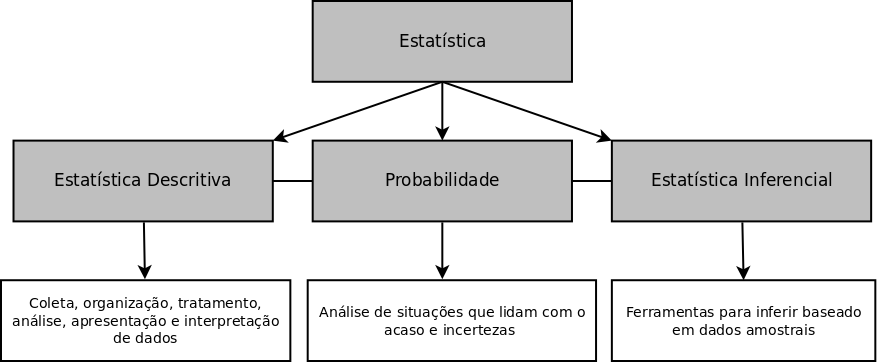
\includegraphics[width=1.0\linewidth]{figs/organograma_estatistica} \end{center}
\blfootnote{\url{http://www.leg.ufpr.br/}}
\end{frame}


\setbeamercovered{transparent}
\begin{frame}
\frametitle{Divisões básicas da estatística}

\begin{center}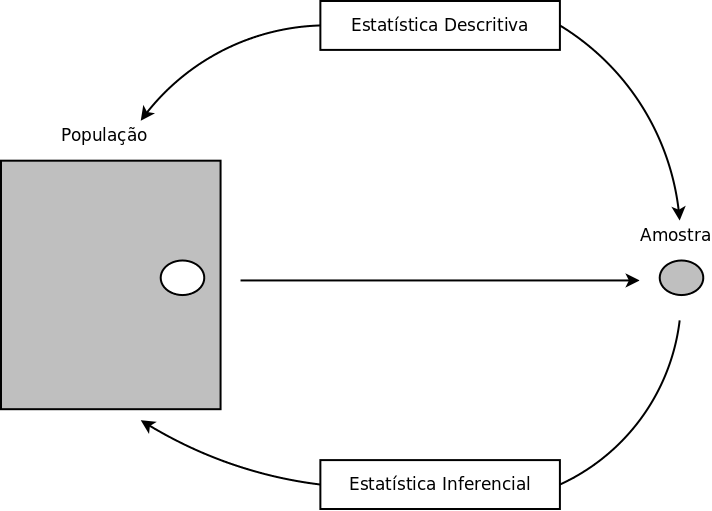
\includegraphics[width=0.75\linewidth]{figs/populacao_amostra} \end{center}
\blfootnote{\url{http://www.leg.ufpr.br/}}
\end{frame}
\section{Revisão - Distribuição Normal}
\setbeamercovered{transparent}
\begin{frame}
\frametitle{Função densidade de probabilidade}

Não podemos atribuir probabilidades à valores específicos, pois há uma
quantidade \textbf{não enumerável} (infinita) de valores em um ponto.

Atribuimos probabilidades à intervalos de valores, por meio de uma
\textbf{função}. Portanto, as probabilidades são representadas por
áreas.


\begin{center}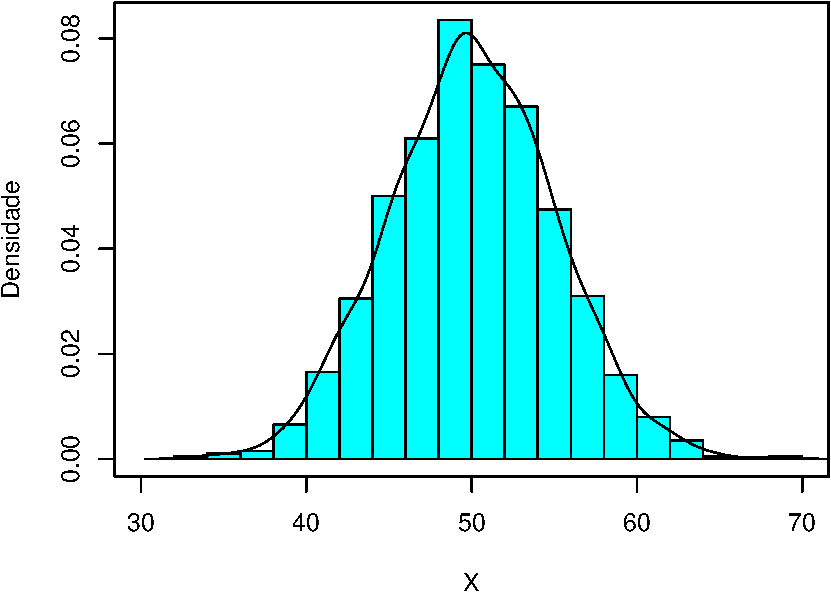
\includegraphics[width=0.55\linewidth]{figs/dens-1} \end{center}
\end{frame}

\setbeamercovered{transparent}
\begin{frame}
\frametitle{Função densidade de probabilidade}

A \textbf{função densidade de probabilidade} (fdp) atribui
probabilidades à intervalos de valores do tipo \([a,b]\), e é definida
por \[
P[a < X < b] = \int_{a}^{b} f(x) dx
\] com as seguintes propriedades:

\begin{enumerate}
\def\labelenumi{\roman{enumi}.}
\item
  É uma função não negativa \[f(x) \geq 0\]
\item
  A área total sob a curva deve ser igual a 1
  \[\int_{-\infty}^{+\infty} f(x) dx = 1\]
\end{enumerate}
\end{frame}

\setbeamercovered{transparent}
\begin{frame}
\frametitle{Modelo Normal}

\textbf{Definição:} Dizemos que uma VA \(X\) segue o modelo normal se
sua fdp é a seguinte \[
f(x) = \frac{1}{\sigma\sqrt{2\pi}} \exp\left[-\frac{1}{2} \left( \frac{x -
\mu}{\sigma}\right)^2\right], \quad -\infty < x < \infty
\] onde \(\mu \in \mathbb{R}\) é a média da população,
\(\sigma \in \mathbb{R}^+\) é o desvio-padrão populacional.

\textbf{Notação:} \(X \sim \text{N}(\mu, \sigma^2)\)

\textbf{Esperança e variância:} \(E(X) = \mu\) e \(Var(X) = \sigma^2\)
\end{frame}

\setbeamercovered{transparent}
\begin{frame}
\frametitle{Modelo Normal}

\begin{center}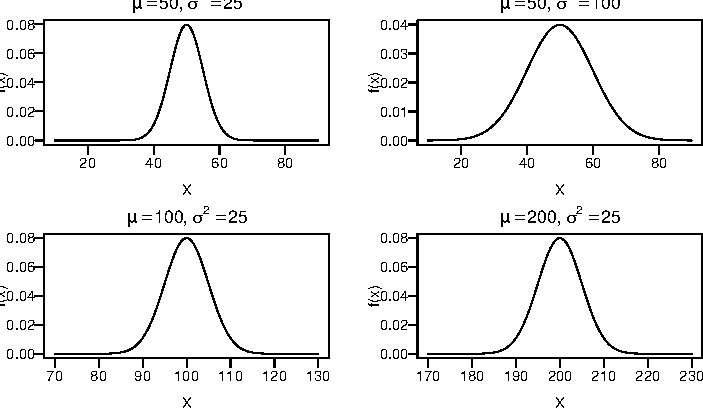
\includegraphics[width=0.99\linewidth]{figs/unnamed-chunk_5_1} \end{center}
\end{frame}

\setbeamercovered{transparent}
\begin{frame}
\frametitle{Modelo Normal}

Característcas da curva normal:

\begin{itemize}
\item
  É \textbf{simétrica} em relação à \(\mu\)
\item
  O ponto máximo (moda) de \(f(x)\) é o ponto \(x=\mu\)
\item
  Os pontos de inflexão da função são \(\mu-\sigma\) e \(\mu+\sigma\)
\item
  A área total sob a curva é 1 ou 100\%
\end{itemize}
\end{frame}

\setbeamercovered{transparent}
\begin{frame}
\frametitle{Modelo Normal}

Para qualquer VA normal \(X\), valem as seguintes relações:
\begin{align*}
&P[X > \mu] = P[X < \mu] \\
&P[\mu - \sigma < X < \mu + \sigma] \approxeq 0,683 \\
&P[\mu - 2\sigma < X < \mu + 2\sigma] \approxeq 0,954 \\
&P[\mu - 3\sigma < X < \mu + 3\sigma] \approxeq 0,997
\end{align*} Portanto, \(6\sigma\) é frequentemente referida como a
\textbf{largura} de uma distribuição normal.

Métodos mais avançados de integração podem ser utilizados para mostrar
que a área sob a função densidade de probabilidade normal de
\(-\infty < x < \infty\) é igual a 1.
\end{frame}

\setbeamercovered{transparent}
\begin{frame}
\frametitle{Regra empírica para uma distribuição normal}

\begin{center}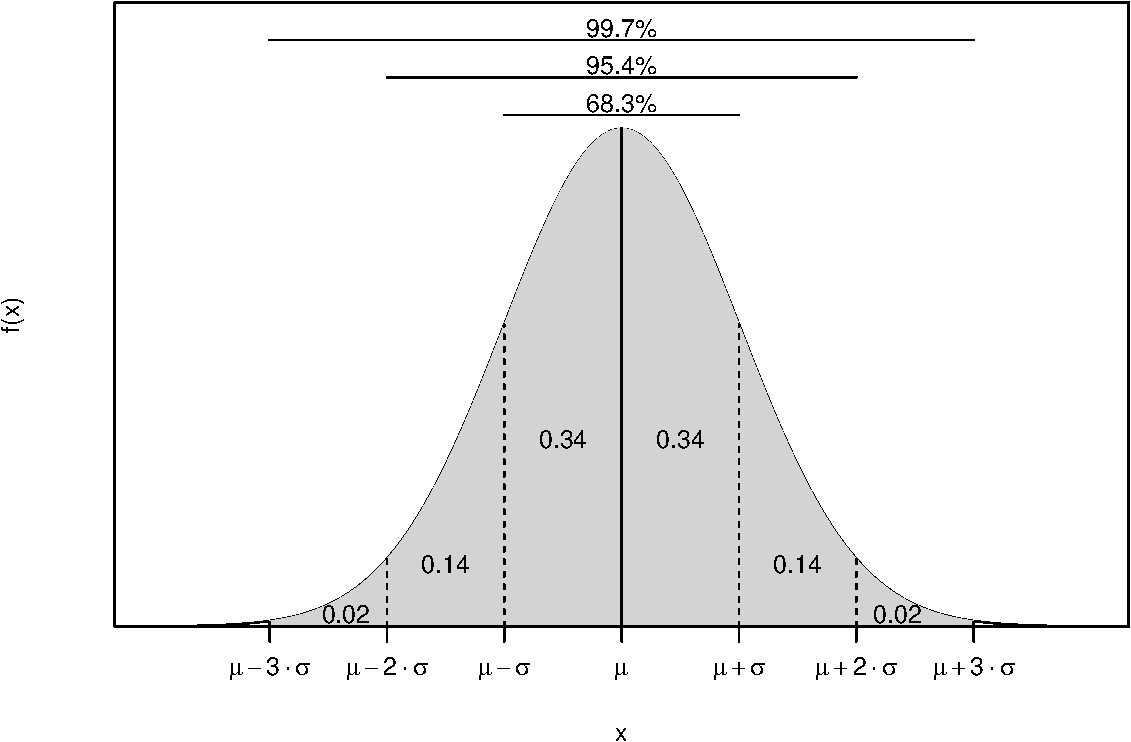
\includegraphics[width=0.9\linewidth]{figs/empnorm-1} \end{center}
\end{frame}

\setbeamercovered{transparent}
\begin{frame}
\frametitle{Modelo Normal}

Para obter uma probabilidade do modelo normal, devemos calcular a área
entre os pontos \(a\) e \(b\), ou seja, \[
P[a < X < b] = \int_a^b \frac{1}{\sqrt{2\pi}\sigma} \exp\left[-\frac{1}{2}
\left( \frac{x - \mu}{\sigma}\right)^2\right] dx
\] No entanto, essa função não possui forma fechada, e o cálculo de
probabilidades pode ser feito apenas por aproximações numéricas.

Para contornar esse problema, os valores de probabilidade são obtidos
para uma distribuição normal padrão (\(Z\)) com \(\mu = 0\) e
\(\sigma^2 = 1\), \[
Z = \frac{X - \mu}{\sigma} \sim \text{N}(0,1)
\] A vantagem é que podemos fazer uma única tabela com as integrais
aproximadas de \(Z\), ao invés de uma tabela para cada par
\((\mu,\sigma^2)\).
\end{frame}

\setbeamercovered{transparent}
\begin{frame}
\frametitle{Modelo Normal}

\begin{center}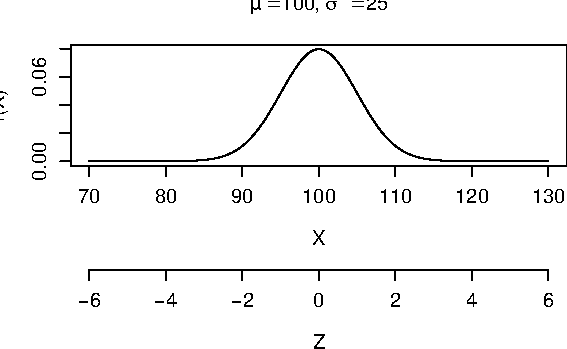
\includegraphics[width=0.8\linewidth]{figs/unnamed-chunk_6_1} \end{center}
\end{frame}


\setbeamercovered{transparent}
\begin{frame}
\frametitle{Exemplo 6.8}

Doentes sofrendo de certa moléstia são submetidos a um tratamento
intensivo cujo tempo de cura foi modelado por uma densidade Normal de
média \(15\) e desvio padrão \(2\) (em dias).

\begin{itemize}
\item
  Calcule a proporção de pacientes que demorarão mais de \(17\) dias
  para se recuperar.
\item
  Calcule a probabilidade um paciente selecionado ao acaso demorar menos
  de \(20\) dias para se recuperar.
\item
  Qual o tempo máximo necessário para a recuperação de 25\% dos
  pacientes?

\end{itemize}
\end{frame}


\end{document}